\begin{center}
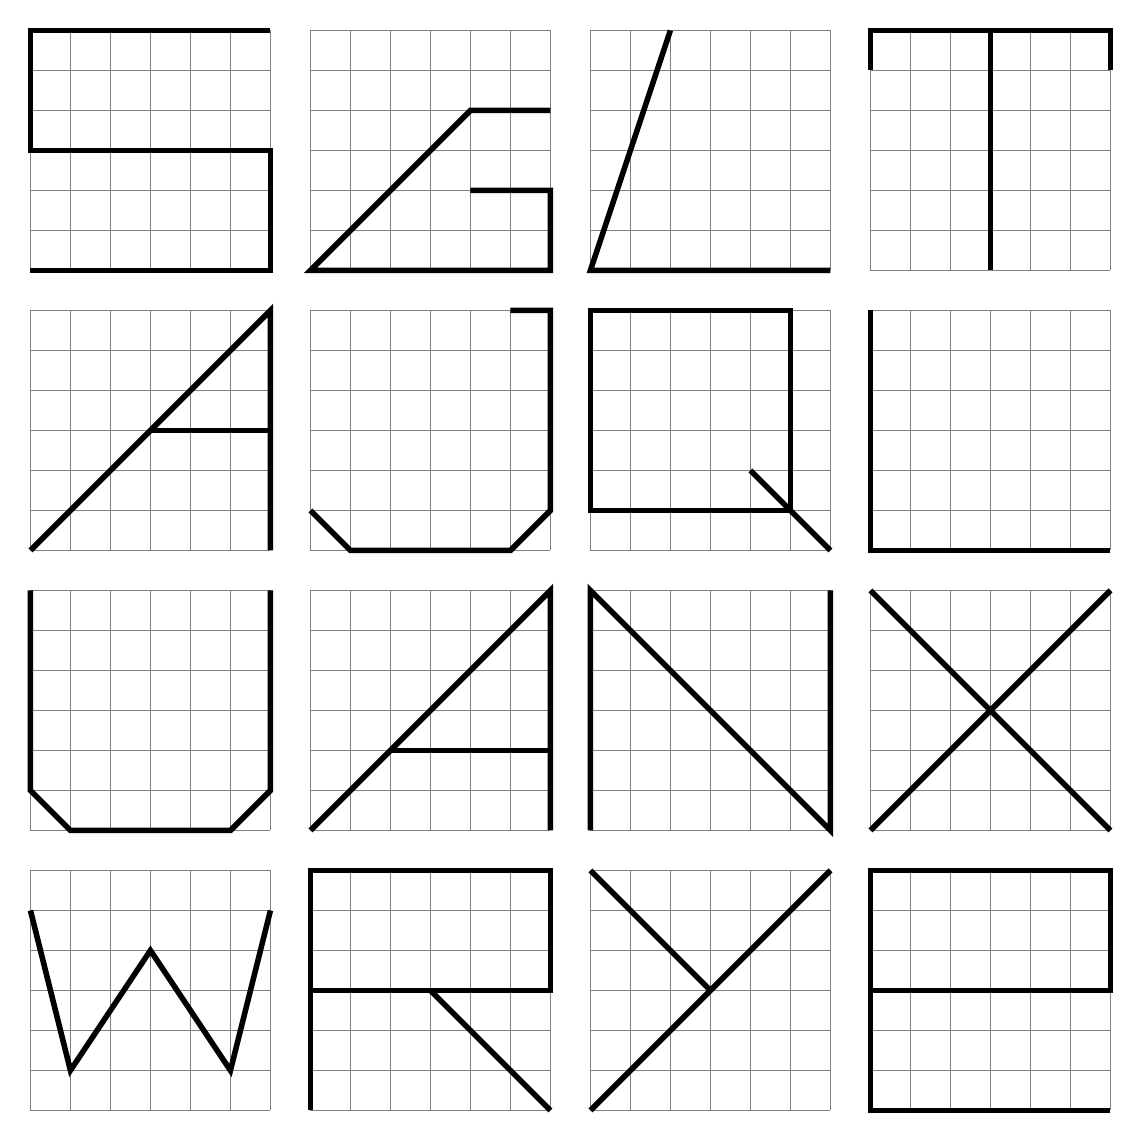
\begin{tikzpicture}[x=0.2in,y=0.2in] 
\begin{scope}[shift={(0,21)}] %BAD S
\fill[white] (0,0) rectangle (6,6);
\draw[step=1,thin,gray] (0,0) grid (6,6);
\draw[line width=2pt] (6,6) -- (0,6) -- (0,3) -- (6,3) -- (6,0) -- (0,0); 
\end{scope} 
\begin{scope}[shift={(7,21)}] %GOOD G
\fill[white] (0,0) rectangle (6,6);
\draw[step=1,thin,gray] (0,0) grid (6,6);
\draw[line width=2pt] (4,2) -- (6,2) -- (6,0) -- (0,0) -- (4,4) -- (6,4);
\end{scope}
\begin{scope}[shift={(14,21)}] %BAD L
\fill[white] (0,0) rectangle (6,6);
\draw[step=1,thin,gray] (0,0) grid (6,6);
\draw[line width=2pt] (2,6) -- (0,0) -- (6,0); 
\end{scope}
\begin{scope}[shift={(21,21)}] %BAD T
\fill[white] (0,0) rectangle (6,6);
\draw[step=1,thin,gray] (0,0) grid (6,6);
\draw[line width=2pt] (6,5) -- (6,6) -- (0,6) -- (0,5);
\draw[line width=2pt] (3,6) -- (3,0);
\end{scope}

\begin{scope}[shift={(0,14)}] %GOOD A(1)
\fill[white] (0,0) rectangle (6,6);
\draw[step=1,thin,gray] (0,0) grid (6,6);
\draw[line width=2pt] (0,0) -- (6,6) -- (6,0);
\draw[line width=2pt] (3,3) -- (6,3);
\end{scope}
\begin{scope}[shift={(7,14)}] %BAD J
\fill[white] (0,0) rectangle (6,6);
\draw[step=1,thin,gray] (0,0) grid (6,6);
\draw[line width=2pt] (5,6) -- (6,6) -- (6,1) -- (5,0) -- (1,0) -- (0,1);
\end{scope}
\begin{scope}[shift={(14,14)}] %BAD Q
\fill[white] (0,0) rectangle (6,6);
\draw[step=1,thin,gray] (0,0) grid (6,6);
\draw[line width=2pt] (0,1) -- (0,6) -- (5,6) -- (5,1) -- cycle; 
\draw[line width=2pt] (4,2) -- (6,0); 
\end{scope}
\begin{scope}[shift={(21,14)}] %GOOD L
\fill[white] (0,0) rectangle (6,6);
\draw[step=1,thin,gray] (0,0) grid (6,6);
\draw[line width=2pt] (6,0) -- (0,0) -- (0,6);
\end{scope}

\begin{scope}[shift={(0,7)}] %BAD U
\fill[white] (0,0) rectangle (6,6);
\draw[step=1,thin,gray] (0,0) grid (6,6);
\draw[line width=2pt] (0,6) -- (0,1) -- (1,0) -- (5,0) -- (6,1) -- (6,6);
\end{scope}
\begin{scope}[shift={(7,7)}] %GOOD A(2)
\fill[white] (0,0) rectangle (6,6);
\draw[step=1,thin,gray] (0,0) grid (6,6);
\draw[line width=2pt] (0,0) -- (6,6) -- (6,0);
\draw[line width=2pt] (2,2) -- (6,2);
\end{scope}
\begin{scope}[shift={(14,7)}] %BAD N
\fill[white] (0,0) rectangle (6,6);
\draw[step=1,thin,gray] (0,0) grid (6,6);
\draw[line width=2pt] (0,0) -- (0,6) -- (6,0) -- (6,6); 
\end{scope}
\begin{scope}[shift={(21,7)}] %GOOD X
\fill[white] (0,0) rectangle (6,6);
\draw[step=1,thin,gray] (0,0) grid (6,6);
\draw[line width=2pt] (0,0) -- (6,6);
\draw[line width=2pt] (0,6) -- (6,0);
\end{scope}

\begin{scope}[shift={(0,0)}] %BAD W
\fill[white] (0,0) rectangle (6,6);
\draw[step=1,thin,gray] (0,0) grid (6,6);
\draw[line width=2pt] (0,5) -- (1,1) -- (3,4) -- (5,1) -- (6,5);
\end{scope}
\begin{scope}[shift={(7,0)}] %BAD R
\fill[white] (0,0) rectangle (6,6);
\draw[step=1,thin,gray] (0,0) grid (6,6);
\draw[line width=2pt] (0,0) -- (0,6) -- (6,6) -- (6,3) -- (0,3); 
\draw[line width=2pt] (3,3) -- (6,0);
\end{scope}
\begin{scope}[shift={(14,0)}] %GOOD Y
\fill[white] (0,0) rectangle (6,6);
\draw[step=1,thin,gray] (0,0) grid (6,6);
\draw[line width=2pt] (0,0) -- (6,6);
\draw[line width=2pt] (0,6) -- (3,3);
\end{scope}
\begin{scope}[shift={(21,0)}] %BAD E
\fill[white] (0,0) rectangle (6,6);
\draw[step=1,thin,gray] (0,0) grid (6,6);
\draw[line width=2pt] (6,0) -- (0,0) -- (0,6) -- (6,6) -- (6,3) -- (0,3);
\end{scope}
\end{tikzpicture}
\end{center}
